\section{Optimal Mechanisms with Both Seller's and Bidder's Cost}

In this section, we take out the constraints and prove that MVAs are optimal in
general. We will also try to find the specific MVA to achieve such optimality,
which turns out to be significantly more complex than previous
simplified case.

The first constraint we are going to remove is seller's cost only.  It's
exciting to introduce bidder's bidding cost since it occurs very often in real
cases and it plays an important role.  Sending emails, making phone calls,
enterring credit card nubmers, depositing money and clicking buttons are all
costly for bidders, though sometimes very tiny.  Bidders may not bid when this
cost is greater than their expected utility. Note that even if the valuation is
very high, the expected utility can be very small because of tense competition,
which is very common in online cases as $n$, the number of potential bidders,
is very large. 

This behaviour (bidders won't bid because of competitions) is very different
compared to that in previous model [cite Sequential Optimal Auctions] of
sequential auctions. In that model, there's a time discount which
makes bidders eager to bid in early rounds with high reserve prices to avoid
waiting lost. That makes a lot sense in some cases but sometimes it may not.
For example, if the seller posts an auction with a very low reserve price in
the first round, most bidders with high valuation must be happy to bid
according to that time discount cost model. But this may not be true. For
example, when I encounter such an auction online \footnote{For example, when I
see a very good item in the Auction House of Diablo III with a very low current
bidding}, I might be very reluctant to bid because there's a big probability
that my bidding will be over taken by someone else's so it's just a waste of
effort. Our cost model can describe this behaviour very well.

Assume an extreme case where the broadcast cost is $0$, the bidder's bidding
cost is $0.1$ and there are $n \rightarrow \infty$ many $[0, 1)$-uniform
distributed bidders. In a Dutch auction (a Dutch auction has infinite many
rounds of broadcasts so we have to set braodcast cost to $0$), only one bidder
is expected to bid (no competition), thus every bidder with a valuation $v_i
> 0.1$ should be benifitable to bid when the reserve price drops to a little
> bit below
$v_i-0.1$ (recall that $n \rightarrow \infty$).  In a Vickrey auction, however,
the competition is very tense. Only bidders with valuation greater than $t$ can
accept such intense competition where $t$ satisfies $t^{n-1}t - 0.1 = 0$ (the
expected utility for a bidder with valuation $t$ is $0$).  Thus $t =
\sqrt[n]{0.1}$ which is arbitrary close to $1$ as $n$ grows to infinity.  Thus
almost all bidders can't bare this competition when $n$ is really large.

So a bad mechanism (e.g. a Vickrey auction) with too much cost will have less
participations and therefore decreases seller's utility significantly.  To see
this, look at previous extrame case again.  The revenue of Dutch auction will
converge to $0.9$ (someone with valuation very close to $1$ will bid for price
very close to $0.9$) when $n$ becomes infinity.  The revenue of a Vickrey
auction, however, is only $\int_t^1 x \, (n-1) \,n\,( 1-x) \,{x}^{n-2} dx$
which converges to about $0.67$ when $n$ grows to infinity.  

Another problem caused by bidder's cost is that revenue equivalence theorem
seems to be no longer applicable. That's not strange as the revenue equivalence
theorem assumes that the utility of a bidder is equal to the valuation minus
the payment. This assumption is no longer true as now the utility is also
influenced by the cost charged to this bidder.

Finally, the byproduct of removing the first constraint (or equivalently allowing
bidder's bidding cost) is that we have to remove our second constraint, the
efficiency of the mechanism, as you may have already observed. Since there's cost
for bidders to bid, we could no longer enforce the mechanism to always allocate
the item to the bidder with highest valuation. If we do so, it will become
infeasible when that highest valuation is less than the bidding cost, i.e. the
expected utility will be negative for some bidders to participate this
mechanism.

In summary, we now introduce bidder's bidding cost and drops efficiency
constraint for our mechanisms. The first issue we are going to solve is to make
revenue equivalence theorem, or a very similar theorem, applicable to our model
again. That's vital for seller's utility maximization.

\subsection{Spending Equivalence Theorem and Revenue Optimization Strategy}

\begin{theorem}\label{theorem:equivalence}

The expected overall spendings from all bidders (including their bidding costs
and payments to the seller) in a feasible mechanism (with our cost model) is
completely determined by the expected utility of lowest type bidders and
allocation probability function
$$p: (v_1, v_2, \ldots, v_n) \rightarrow (p_1, p_2, \ldots, p_n)$$ 
where $p_i$ is the probability that bidder $i$ will get the item.

\end{theorem}

\begin{proof}
This theorem is exactly the same as revenue equivalence theorem except
that we exchange revenue with spending. To prove it,
let's construct another mechanism $M'$ (from our mechanism $M$) that fits into the original revenue equivalence
theorem's model. Suppose there's a virtual seller in $M'$, who collects valuations from all
bidders at no cost (a direct revelation mechanism). Then this virtual seller will
make $n$ virtual bidders delegating all bidders to communicate with the true seller in our mechanism $M$.
When our mechanism ends by allocating the item to virtual bidder $i$, the virtual seller also
allocate the item to the real bidder $i$. The payment from each bidder $i$ to this
virtual seller will be equal to the payment that virtual bidder $i$ pays to our real seller
plus all the bidding costs charged to virtual bidder $i$. Thus, from the real bidders'
aspects, this mechanism $M'$ is just a direct revelation mechanism which will satisfy
revenue equivalence theorem. The only difference is that the payment from real bidder $i$ to the virtual seller
actually has two parts, one is payed to the real seller, another is payed to bidding costs, which sum
up to the total spending.
\end{proof}

Thanks to theorem \ref{theorem:equivalence}, our revenue maximization problem
is now greatly simplified: we only need to determine optimal allocation rule
$p: (v_1, v_2, \ldots, v_n) \rightarrow (p_1, p_2, \ldots, p_n)$ and the minimum
cost given that allocation rule. However, the optimal allocation rule here
isn't as simple as the one that's discovered by Myerson [ref:Optimal Auction]:
allocate the item to the bidder with highest virtural value if it's positive.
This rule, though optimal in Myerson's setting, may not be optimal here. Theorem
\ref{theorem:equivalence} tells us that this rule will maximize the total spending.
But we must substract the cost from the spending to get the revenue. Therefore,
can there be another weird allocation rule that has less total spending but even
much less minimum cost, so a greater revenue is achieved by that allocation rule.

It's not hard to find one example to support our suspicion. We know that for bidders
with uniform valuation over $[0, 1)$, the spending maximizing allocation rule
is allocate the item to the bidder with highest valuation that's greater than $1/2$.
However, if the broadcast is too large, for example $1$ (which is equal to the
highest possible valuation), the cost to find out whether there's any bidder with valuation
greater than $1/2$ is at least $1$. Thus if we use this allocation rule, the
final revenue would be negative since the total spending must be less than the
minimum cost. However, the allocation rule that never allocate the item will have
$0$ cost and $0$ spending, which achieves $0$ revenue, better than previous allocation
rule.

Thus, the revenue optimal mechianism will depend on how minimum cost is defined. 
We previously defined how cost is charged and proved that a specific mechanism (MVA)
has minimum cost when allocation rule is allocate efficiently. But unfortunately,
that's not enough to give us a well defined minimum cost for any allocation rule.
For example, one allocation rule might be always allocate the item to each bidder
with the same probability $1/n$, i.e. $p(v_1, v_2, \ldots) = (1/n, 1/n, \ldots)$.
You might think that the minimum cost for this is $0$ since we don't have to know
anyone's valuation. But that cost isn't realistic: how can you ever allocate the
item to someone that you have never communicated with? Thus the minimum cost seems
to be at least $b$, the cost for one round of broadcast, if we ever allocate the item
to some bidder. In order to make a realistic constraint and get a well defined minimum
cost for any allocation rule, we define

\begin{definition}\label{def:allocation_cost}
For an allocation rule $$p: (v_1, v_2, \ldots, v_n) \rightarrow (p_1, p_2,
\ldots, p_n)$$ if $p_i > 0$ for some valuation profile $(v_1, v_2, \ldots,
v_n)$, there must be a broadcast query that the $i$-th bidder with valuation
$v_i$ reply to the seller under that profile setting.
\end{definition}

With this definition, we have

\begin{theorem}
The optimal mechanism should always allocate the item to the bidder with
highest virtual valuation $v_i - \frac{1-F(v_i)}{f(v_i)}$ if it decides to
allocate the item. In regular cases when the virtual valuation is monotone
strictly increasing, the optimal mechanism should always allocate the item to
the bidder with highest valuation if it decides to allocate the item.
\end{theorem}

To see why this theorem holds, firstly notice that in our cost model, the
minimum cost to let any bidder reply is equal to the minimum cost to let the
max-valuation bidder (or max-virtual-valuation bidder, we won't mention virtual
valuation below because they are indifferent in our cost context so you can
always substitude one by another, adding or removing regularity constraint)
reply.  This is because that the mechanism is only allowed to ask broadcast
queries and it's equivalent to specify a range $Q \subseteq [0, 1)$ and ask all
bidders whose valuations are within that range to reply. That means, by
properly mappings of valuations and query ranges, we can always adapt a
strategy that lets any bidder reply to another strategy that lets the
max-valuation bidder reply and vise versa (just like what we did to prove lemma
\ref{lemma:descending}). This means that finding the max-valuation bidder won't
cost more than any other cases except doing nothing (which costs $0$). Thus the
optimal mechanism either do nothing (no one replies and thus $p_i = 0$ by
definition \ref{def:allocation_cost}) which has minimum cost or ask queries to
find the max-valuation bidder and allocate the item to that bidder which has
maximum total spending.  The flexibility of an optimal mechanism is that it can
choose the cases in which it won't allocate the item (in any other cases it
will allocate the item to the max-valuation bidder). It's also intuitive
to see that the no allocation cases can be described by a single parameter $l$:
no allocation if every bidder's valuation is below $l$. For limit of space,
we won't list the detailed proof for the above theorem and arguments.

Now we can narrow our optimal mechanisms with relaxed efficiency constraint:

\begin{definition}

We say mechanisms satisfy relaxed efficiency constraint with low value $l$
if:

    \begin{enumerate}

    \item They only allocate the item to bidders whose valuation are at least
    $l$ (the low value is $l$)

    \item If they will allocate the item, they will always allocate the item to
    the bidder with highest valuation.

    \end{enumerate}

When we say a mechanism with a low value $l$, we imply that this mechanism
satisfy relatex efficiency constraint with lowest $l$.

\end{definition}

\subsection{Cost Minimization with Low Value and MVAs' Optimality in General}

We have already narrowed down optimal mechanism to
relatex efficient mechanisms and by theorem \ref{theorem:equivalence},
it's straightforward to see

\begin{corollary}

For mechanisms with a fixed low value $l$, the maximum utility for sellers is
achieved when the mechanism minizes the cost.

\end{corollary}

Our next question is naturally: what's the cost minimized mechanism
given a low value $l$. As expected:

\begin{theorem}

MVAs have the minimum cost among all mechanisms with a low value $l$

\end{theorem}

\begin{proof}
A special case of this theorem when $l = 0$ is theorem \ref{theorem:MVA_eq}.
We proved that special case by introducing lemma \ref{lemma:uniform} and
\ref{lemma:descending}. To prove the general cases with arbitrary $l$, we just
need to revise lemma \ref{lemma:uniform} a little as following lemma
\ref{lemma:lowest_type}. All other part of the proof remains similar. For space
limit, the detailed proof is omitted.
\end{proof}

\begin{lemma}\label{lemma:lowest_type}
Suppose that there are two cases $n, F_1, f_1, l_1$ and $n, F_2, f_2, l_2$
where $n$ is the number of values for both cases, $F_i, f_i$ are CDF and PDF
of the $n$ i.i.d. values in case $i$, $l_i$ is the low value for case $i$.
If $F_1(l_1) = F_2(l_2)$, then these two cases have the same minimum cost
to find the maximum value above the low value $l_i$.
\end{lemma}

The proof of this revised lemma is almost identical to the one for original
lemma. Thus for space limit, we won't elaborate it again. Finally, we conclude
that MVAs are optimal in general.

\begin{corollary}

MVAs are optimal. The only parameters we are going to determine for the
specific optimal MVA are 1) the low value $l$; 2) the descending query
thresholds $q_1, q_2, q_3, \ldots$.

Shall we increase low value $l$ a little above Myerson's optimal low value
to trade payment with cost? Or is it optimal to use Myerson's $l$ and then
minimize cost according to that?

\end{corollary}

\subsection{Experiments to Discover Optimal MVA with a Given Low Value}

To discover the specific MVA that's optimal, we first try to identify the
optimal thresholds $a_i$ given a low value $l$  (recall that in $i$-th round,
MVA will ask all bidders whose valuation is within $[a_i, a_{i-1})$ to bid).
If we can write the minimum cost $C^*$ as a function of $n, \rho, l$ (recall
that $rho = b/c$ is the ratio between broadcast and bidding cost), we may then
determine the optimal $l$ using this function.

In the special case that we studied in previous section where $l = 0$
(efficiency is enforced), the optimal thresholds can be easily described as a
single parameter $\alpha$. This strategy won't work when $l > 0$ (more
precisely, $F(l) > 0$, but because of lemma \ref{lemma:lowest_type}, we only
focus on uniform distribution in the following). Obviously that $a_i \geq l$,
thus we can't let $a_i = \alpha a_{i-1}$ since $\lim_{i \rightarrow \infty} a_i
= 0 < l$.  Additionally, if we revise the equation by letting $a_i-l = \alpha
(a_{i-1}-l)$, we will get a positive possibility $F(l)$ that we would ask
infinite many broadcast queries, which is even worse.

As it's not immediately clear what optimal thresholds should be like, we
present a simple algorithm to calculate such thresholds numerically. We firstly
discretize the continuous valuation $[0, 1)$ to $D$ discrete values $\{0, 1, \ldots,
D-1\}$. That means, the original valuation $v$ will be transformed to integer
value $\hat v = \lfloor v D \rfloor$. Then we use dynamic programming to
inductively calculate $x_{\hat r}$, the length of next optimal descending query to ask
(therefore the query would be $[\hat r-x_{\hat r}, \hat r)$), conditional on that we have
already queried $[\hat r, D)$ and no one replies.

\begin{algorithm}
    \caption{Calculate discretized best query lengths}\label{algo:discrete}
    \begin{algorithmic}[1]
        \Require{$\hat l$ is the discretized low value, $\rho$ is the ratio between broadcast and bidding cost,
        $n$ is the number of bidders, $D$ is the maximum discretized valuation}
        
        \Function{BestQueryLengths}{$\hat l$, $\rho$, $n$, $D$}
            \State $x_{\hat l} \gets 0$
            \State $C_{\hat l} \gets 0$
            \For{$\hat r={\hat l}+1 \mbox{ to } D$}
                \State $x_{\hat r} \gets \displaystyle
                  \operatorname*{arg\,min}_{1 \leq x \leq \hat r-l} \rho + n
                  \frac{x}{\hat r} + (\frac{\hat r-x}{\hat r})^n C_{\hat r-x}$
                \State $C_{\hat r} \gets \rho + n \frac{x_{\hat r}}{\hat r} +
                  (\frac{\hat r-x_{\hat r}}{\hat r})^n C_{\hat r-x_{\hat r}}$
            \EndFor
            \State \Return $x$
        \EndFunction
    \end{algorithmic}
\end{algorithm}

Algorithm \ref{algo:discrete} runs in time $O(D^2)$. Having $x$, we can then
infer the best strategy for original continuous problem by first discretize it
and then convert the discretized optimal strategy back to continuous strategy.
The larger $D$ is the more accurate it will be. But it will also require more
running time.  Running this for case $\hat l = 500, \rho = 2, n = 10, D = 1000$
we get $x$ showed in figure \ref{fig:x-r}. It seems that $x$ is a piecewise
linear function over $\hat r$.  For those $\hat r$ which is close to $\hat l$, obviously
that the optimal strategy should be $x = \hat r-\hat l$, which means using only one
query to explore all potential bidders. But it's unclear why $x$ is linear when
the best strategy is using multiple queries to explore the valuation range.

\begin{figure}
\centering
    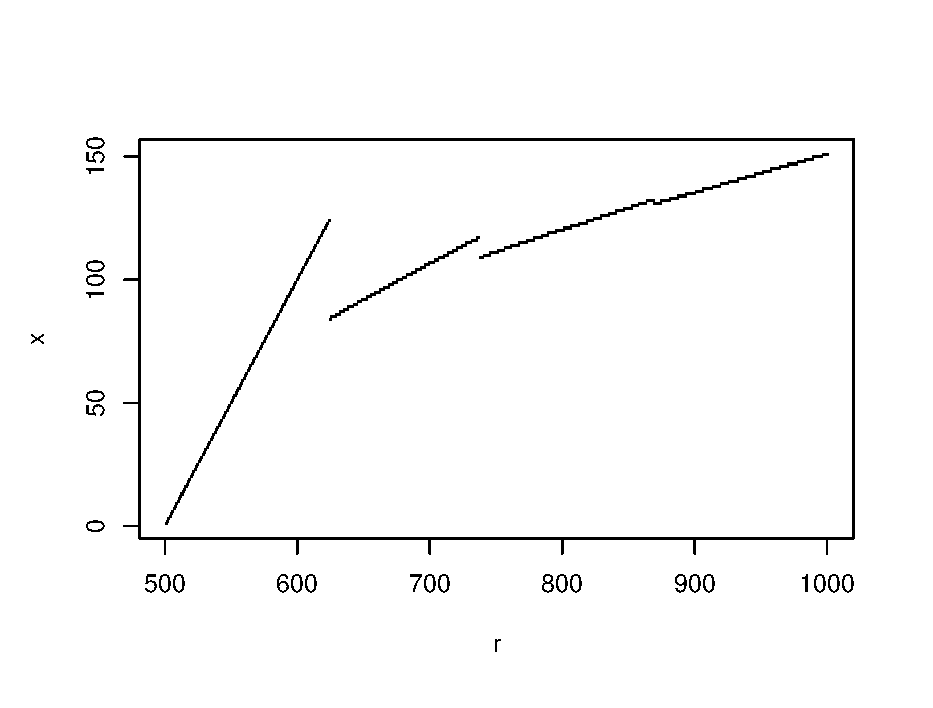
\includegraphics[trim=0mm 5mm 5mm 15mm, clip, width=\linewidth]{figures/1000-500-2-1-10}
    \caption{The best query lengths over $r$ (the upper bound of
        undiscovered value) when discretized low value $\hat l = 500$,
        ratio between broadcast and bidding cost $\rho = 2$,
        number of bidders $n = 10$ and maximum discretized valuation
        $D = 1000$}\label{fig:x-r}
\end{figure}

\subsection{Analysis of Optimal MVA with a Given Low Value}

Figure \ref{fig:x-r} shows that the optimal MVA with a low value $l$ is
much more complicated but there might still be hope to get a nice analytical
result: piecewise linear function. That is, we can't use a single $\alpha$ to
describe such optimal MVA, but perhaps we can use a sequence of $\alpha$ to
describe it. Now let's take an analytical treatment.

The first key point to analyze the optimal MVA with low value is to utilize
the fact that there's a fixed maximal number of rounds to exploit the whole
reportable valuation range $[l, r)$ ($r$ is the upper bound of undiscovered
value as defined in last subsection and $r = 1$ initially). Let's call that
number $k$. We have argued this before: if not, because the possibility that no
values lie in $[l, r)$ is possitive, the cost will be infinte.

For convenience, define $\vec a = (a_0, a_1, a_2, \ldots, a_k)$, the vector of
$k$ thresholds in such optimal MVA. We make $a_0 = r, a_k = l$ so in $i$-th
round the query would be $[a_i, a_{i-1})$. Now define cost $C(\vec a, k, \rho,
n)$ to be the expected cost for MVA defined by $k, \vec a$ when there are $n$
i.i.d.  $[0, 1)$-uniform bidders (note that $l, r$ are implicitly defined by
$a_k, a_0$). If we can get a neat form of $C$, we can use $\frac{\partial
C}{\partial a_i} = 0 $ to characterize optimal MVA, as we did in section
\ref{sec:alpha-MVA}.

Thus the second key point is to how to represent this $C$. Rather than
considering one round after another as we did before, now we consider all
rounds together:
\begin{align*}
C(\vec a, k, \rho, n) =
&\sum_{i=0}^k P\big(H_i = 1\big) C\big(\vec a, k, \rho, n ~\big|~ H_i = 1 \big)
\end{align*}
where $H_k$ is the indicate random variable for the event that the highest
valuation is below $a_k$ and $H_i(0 \leq i < k)$ is for the event that the highest
valuation is in $[a_{i+1}, a_i)$.

Since bidders are uniformly distributed,
\begin{align*}
  &P(H_k = 1) = a_k^n / a_0^n\\
    &P(H_i = 1) = (a_{i}^n-a_{i+1}^n) / a_0^n
\end{align*}

It's also clear that $C(\vec a, k, \rho, n ~\big|~ H_k = 1) = k\rho$ because
there will be only $k$ broadcasts and no biddings.

For $C\big(\vec a, k, \rho, n ~\big|~ H_i = 1\big)$ where $i < k$, we partition
it into two parts $C\big(\vec a, k, \rho, n ~\big|~ H_i = 1\big) = C_b\big(\vec
a, k, \rho, n ~\big|~ H_i = 1\big) + C_c\big(\vec a, k, \rho, n ~\big|~ H_i =
1\big)$. The broadcast part $C_b\big(\vec a, k, \rho, n ~\big|~ H_i = 1 \big)$
is simply $(i+1)\rho$ as the MVA finishes in $(i+1)$-th round. The
not-so-obvious part is the overall bidding cost $C_c\big(\vec a, k, \rho, n
~\big|~ H_i = 1 \big)$. It can be expressed as:

\begin{align*}
P(H_i = 1)C_c\big(\vec a, k, \rho, n ~\big|~ H_i = 1 \big) = E\left( H_i \cdot
    \sum_{j=1}^n X_{ij}\right) \\
= E\left( \left( \prod_{j=1}^n B_{ij} \right) \cdot \left(\sum_{j=1}^n X_{ij}
    \right) \right)
\end{align*}

Here $X_{ij}, A_{ij}$ are both indicate random variables of bidder $j$'s valuation $v_j$:
$$
X_{ij} = \begin{cases}
    0, &\mbox{if $v_j \notin [a_{i+1}, a_{i})$ } \\\\
    1, &\mbox{if $v_j \in [a_{i+1}, a_{i})$}
\end{cases}
~~
B_{ij} = \begin{cases}
    0, &\mbox{if $v_j \geq a_{i}$ } \\\\
    1, &\mbox{if $v_j < a_{i}$}
\end{cases}
$$

You may notice that our original random variable $H_i$ is not exactly the same
as our substitute $\prod_{j=1}^n B_{ij}$. The only difference between them,
however, is the case that every $v_j$ is below $a_{i+1}$, which is the case
that every $X_{ij} = 0$, so the equation still holds.

Now we use the properties of expectation to finish our calculation:
\begin{align*}
  &E\left( \left( \prod_{j=1}^n B_{ij} \right) \cdot \left(\sum_{j=1}^n X_{ij}
  \right) \right) = \sum_{j=1}^n E\left( X_{ij} \prod_{k=1}^nB_{ik} \right)
  \\
    &~~ = \sum_{j=1}^n \left( E(X_{ij} B_{ij}) \prod_{k \neq j} E(B_{ik})
    \right)
       = n a_{i}^{n-1} (a_{i}-a_{i+1}) / a_0^n
\end{align*}
Combine all those above, finally we get (note that low value $l = a_k$):
\begin{align}
& C(\vec a, k, \rho, n) = k \rho a_k^n / a_0^n + \nonumber\\ 
    &~~~ \frac{1}{a_0^n} \sum_{i=0}^{k-1} \left( (a_{i}^n-a_{i+1}^n) (i+1)
    \rho + n a_{i}^{n-1} (a_{i}-a_{i+1}) \right) \label{eq:C_general}
\end{align}

Unfortunately, this formula isn't neat enough to get a piecewise linear $a_1$.
Recall that in previous subsection, the experiment seems to show that $x$ is
piecewise linear over $r$, which means $a_1$ must also be piecewise linear over
$a_2$.  For example, for the simple case $k = 2, n = 3$, we have: $a_1 =
\frac{\sqrt{{a_0}^{2}\,\rho+{a_2}^{2}+3\,{a_0}^{2}}+a_2}{\rho+3}$.  Anyway,
by definition we have $a_1 \geq a_2$. And
$a_1=\frac{\sqrt{{a_0}^{2}\,\rho+{a_2}^{2}+3\,{a_0}^{2}}+a_2}{\rho+3}$ indeed
looks very linear when $a_1 \geq a_2$.

Though we failed characterizing the optimal MVA using piecewise linear
descriptions, those experiments and analysis may still benefit us. Firstly, the
experiments shows that a piecewise linear MVA might be a nice approximation.
Secondly, the analysis may help us find a better numerically algorithm to
calculate the optimal MVA. For example, an iterative algorithm like EM
algorithm.

\subsection{Using Piecewise Linear MVA to Approximate Optimal MVA}

\subsection{Choosing Low Value?}

\subsection{Experiments}

Now we are going to compare revenue in general cases. We not only compare our
approximate optimal MVAs to optimal MVAs computed numerically, but also compare
MVAs to other conventional mechanisms.


